\documentclass[parskip=half-]{scrartcl}
\usepackage[UKenglish]{babel}
\usepackage{libertine}
\usepackage[T1]{fontenc}
\usepackage[latin1]{inputenc}
\usepackage{tikz}
\usepackage{hyperref}

\title{TeXnicCenter with Sumatra PDF}
\author{Based on a tutorial by\\
Martin Hehn\thanks{martin.hehn@manchester.ac.uk}\\
Updated and corrected by\\
Benjamin Danowski\thanks{benjamin.danowski@web.de}}
\date{\today}

\begin{document}
\maketitle
\tableofcontents
\section{Short Introduction}
This tutorial describes the use of Sumatra PDF viewer (v 1.0.1) in combination with TeXnicCenter (v 1.0).

After successful setup Sumatra PDF recognizes changes in the PDF file which results from repeated compilation in TeXnicCenter (TC) and updates its document view automatically. You do not have to close and restart the program by hand every time. By pressing the F5 button in TC Sumatra PDF shows the page and the section the cursor resides in. Sumatra comes to the front by doing this.\\
\textbf{Please note:} Currently forward search only works if the file name and its whole path do not contain spaces!

A double click in Sumatra PDF should place TCs cursor to the corresponding section. TC comes to the front by doing this.

\section{Software}

\begin{description}
	\item[Sumatra] Download Sumatra PDF 1.0.1 at \url{http://blog.kowalczyk.info/software/sumatrapdf/index.html} 
	\item[TeXnicCenter] Download the latest release (v 1.0). (\url{http://www.texniccenter.org/})
	\item[Distribution] It is assumed that you have a \LaTeX\ distribution already installed, e.g. MiKTeX 2.8 (\url{http://miktex.org/}).\\
TeX Live 2008 (\url{http://www.tug.org/texlive/}) also does the job. However, TeX Live 2008 is distributed with a buggy version of the \texttt{SyncTeX} parser, therefore you have to update the following files:
\begin{itemize}
	\item \texttt{pdftex.dll},
	\item \texttt{pdftex.exe} und
	\item \texttt{kpathseaxxx.dll}
\end{itemize}
They can be downloaded at \url{http://www.tug.org/svn/texlive/trunk/Master/bin/win32/}. \texttt{xxx} stands for a 3-digit number. If you have downloaded a wrong version, you will notice it. After this you want to update the format files by using the TeX Live manager.\\
If you have information about TeX Live 2009 please do not hesitate to tell me your findings.
\end{description}

\section{Settings in Sumatra PDF}
Since version 0.9.4 no changes are neccessary. The command line is delivered by TC. If you made a mistake it could be neccessary to delete the configuration file in the Sumatra PDF folder and the \texttt{.synctex} file corresponding to your source file.
%Open up Sumatra and go to:

%\begin{tikzpicture}
%\node (a) at (0,0) {\texttt{File}};
%\node (b) at (5,-1) {\texttt{Set inverse search command-line}};
%\node (c) at (0,-1) {};
%\draw [-] (a.south) -- (c.center) -- (b.west);
%\end{tikzpicture}

%Insert the following code (Path names may vary):\\
%\verb+"C:\Programme\TeXnicCenter\TEXCNTR.EXE" /ddecmd "[goto('%f','%l')]'"+

\section{Settings in TeXnicCenter}
It is useful to define an extra output profile for Sumatra:

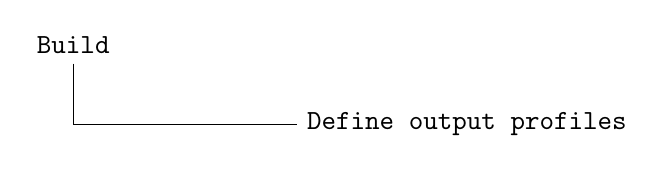
\begin{tikzpicture}
\node (a) at (0,0) {\texttt{Build}};
\node (b) at (5,-1) {\texttt{Define output profiles}};
\node (c) at (0,-1) {};
\draw [-] (a.south) -- (c.center) -- (b.west);
\end{tikzpicture}

\begin{enumerate}
	\item Click in the existing profile \texttt{LaTeX$=>$PDF} 
	\item Click \texttt{Copy}
	\item Name the new profile, e.g. \texttt{LaTeX$=>$PDF (Sumatra)}
\end{enumerate}

Check that the new profile is highlighted. There are three tabs: \texttt{(La)Tex}, \texttt{Postprocessor} and \texttt{Viewer}.

\textbf{(La)Tex}\\
Quickly check if the compiler path is correct (path names may vary)\\
\verb+"C:\Program Files\MiKTeX 2.7\miktex\bin\pdflatex.exe"+

At \texttt{Command line arguments to pass to the compiler} insert the following\\
\verb+-synctex=-1 -interaction=nonstopmode "%Wm"+

\textbf{Postprocessor}\\
No settings required.

\textbf{Viewer}\\
At \texttt{Path of executable} insert the following line (path names may vary):\\
\verb+"C:\Program Files\SumatraPDF\SumatraPDF.exe" -inverse-search+\\ \verb+"\"C:\Program Files\TeXnicCenter\TEXCNTR.EXE\" /ddecmd \"[goto('%f','%l')]\""+

\textbf{NOTE:} There is a space after \texttt{search}, the command was just split into two lines to fit on the page. Furthermore, please do not forget to include the quotation marks if you have spaces in the pathname (e. g. ``Program Files'' on English systems).

At \texttt{View project's output} set the radiobutton to \texttt{Command line argument}

For \texttt{Command:} enter:\\
\verb+"%bm.pdf"+

At \texttt{Forward search} set the radiobutton to \texttt{DDE Command} 

At \texttt{Command:} insert\newline
\verb|[ForwardSearch("%bm.pdf","%Wc",%l,0,0,1)]|\\
\texttt{Server:} \texttt{SUMATRA}\\
\texttt{Topic:} \texttt{Control}

At \texttt{Close document before running (La)TeX} set the radiobutton to \texttt{Do not close}.\\
\\
If you like to read about the Sumatra PDF DDE commands:\\
\\
\url{http://code.google.com/p/sumatrapdf/wiki/DDEcommands}

\section{Important advice}
\begin{itemize}
	\item \textbf{Again:} Currently forward search only works if the file name and its whole path do not contain spaces!
	\item \textbf{Beware:} If you copy the command lines and paths from e.g. Adobe Reader an apostrophe (right) gets an accent (wrong). This breaks functionality. Therefore you have to replace the accents with apostrophes (the key above the ``Enter''-key).\\
	However, after some feedback from users it seems to depend on the configuration of the system the viewer runs on.
	\item User advice also showed that a re-start of TC may be neccessary to activate the changes. So you have to find out yourself.
	\item Furthermore you should use \verb\include\ for embedding other \TeX files. If you use \verb\input\ you have to append the file ending (e.g. myfile.tex).
\end{itemize}


\rule{40pt}{2pt}\\
Enjoy

\section{Version history}
11.08.2009: First version\\
\\
23.09.2009: Included user advice from C. Wiethoff concerning re-start and copy\&paste behaviour of existing PDF viewers. Included advice on spaces in path names.\\
\\
01.10.2009: Got a hint from C. A. Vallejo Pinto how to change configuration so that Sumatra PDF comes to the front by pressing ``F5''. Added link to Sumatra PDF DDE commands.

03.03.2010: PDF viewer behaviour, minor changes, changed advise concerning \verb\include\, quotation marks in the pathname, MiKTeX 2.8, TeX Live 2009

Thanks for feedback!
\end{document}